\documentclass[fontsize=11pt,a4paper,final]{scrartcl}[2003/01/01]
\usepackage[ngerman]{babel} 
\usepackage[utf8]{inputenc} 
\usepackage[autostyle=true,german=quotes]{csquotes}
\usepackage[T1]{fontenc}
\usepackage{float}
\usepackage{floatflt}
\usepackage{listings}
\usepackage[hidelinks]{hyperref}
\usepackage{tabularx}
\usepackage[sort&compress,numbers]{natbib}
\usepackage{caption}
\usepackage{listings}
\usepackage{color}

\captionsetup[table]{skip=0pt}
\captionsetup[figure]{skip=10pt}

\title{Embedded Systems Dokumentation}
\author{Von Christian Weber und Manuel Wurth}
\date{\today}

%Bilder scalen, wenn größer als Seite
\usepackage[final]{graphicx}
\makeatletter
\def\ScaleIfNeeded{%
	\ifdim\Gin@nat@width>\linewidth
		\linewidth
	\else
		\Gin@nat@width
	\fi
}
\makeatother

\newcommand*{\quelle}{% 
	\footnotesize Quelle: 
}

\newcommand*{\manu}{%
	Programmiert von: Manuel Wurth
}

\newcommand*{\chris}{%
	Programmiert von: Christian Weber
}

\lstset{
  backgroundcolor=\color{white},   % choose the background color; you must add \usepackage{color} or \usepackage{xcolor}
  basicstyle=\footnotesize,        % the size of the fonts that are used for the code
  breakatwhitespace=false,         % sets if automatic breaks should only happen at whitespace
  breaklines=true,                 % sets automatic line breaking
  captionpos=b,                    % sets the caption-position to bottom
  commentstyle=\color{mygreen},    % comment style
  deletekeywords={...},            % if you want to delete keywords from the given language
  escapeinside={\%*}{*)},          % if you want to add LaTeX within your code
  extendedchars=true,              % lets you use non-ASCII characters; for 8-bits encodings only, does not work with UTF-8
  frame=single,	                   % adds a frame around the code
  keepspaces=true,                 % keeps spaces in text, useful for keeping indentation of code (possibly needs columns=flexible)
  keywordstyle=\color{blue},       % keyword style
  language=Octave,                 % the language of the code
  otherkeywords={*,...},           % if you want to add more keywords to the set
  numbers=left,                    % where to put the line-numbers; possible values are (none, left, right)
  numbersep=5pt,                   % how far the line-numbers are from the code
  rulecolor=\color{black},         % if not set, the frame-color may be changed on line-breaks within not-black text (e.g. comments (green here))
  showspaces=false,                % show spaces everywhere adding particular underscores; it overrides 'showstringspaces'
  showstringspaces=false,          % underline spaces within strings only
  showtabs=false,                  % show tabs within strings adding particular underscores
  stepnumber=1,                    % the step between two line-numbers. If it's 1, each line will be numbered
  stringstyle=\color{mymauve},     % string literal style
  tabsize=2,	                   % sets default tabsize to 2 spaces
  caption=\lstname                   % show the filename of files included with \lstinputlisting; also try caption instead of title
}

\lstdefinestyle{framed}
{
	frame=lrb,
}

\begin{document}
	
\maketitle
\newpage
\tableofcontents
\newpage

\section{Simulator}
Weil die Gruppenzahl zu hoch ist, als dass ausreichend oft auf die Hardware zugegriffen werden könnte, haben wir uns entschlossen die Anlage zu simulieren. Als erstes wurde ein C-Simulator geschrieben, allerdings hat sich nach einiger Zeit herausgestellt, dass dieser für eine genauere Analyse von Fehlern unvorteilhaft ist. 
Deshalb wurde die Entwicklung nach einiger Zeit eingestellt und ein Java-Simulator mit grafischer Oberfläche entwickelt.

\lstinputlisting{Stop.c}


\subsection{C-Simulator (verworfen)}
\manu

\begin{figure}[H]
	\centering
	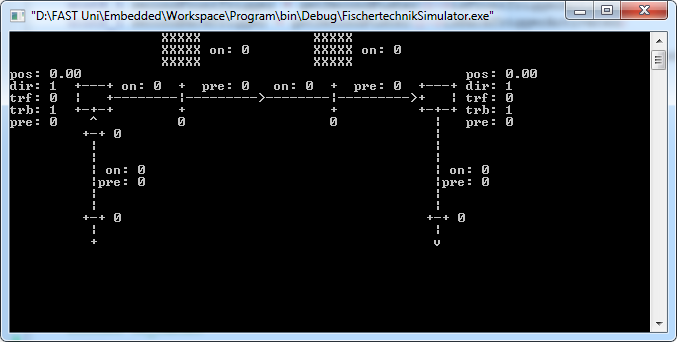
\includegraphics[width=1\ScaleIfNeeded]{Bilder/C-Simulator.png}
	\caption{Der C-Simulator}
	\label{fig:C-Simulator}
\end{figure} \ \\
\noindent Die Ausgabe des Simulators ist in Abbildung \ref{fig:C-Simulator} dargestellt. Ziel war es, die Anlage mit allen relevanten Informationen mithilfe von ASCII-Zeichen darzustellen. Darunter alle Lichtschranken, \textit{Flags}, die anzeigen ob eine Station gerade belegt ist (pre), die beiden Pusher mit ihren Daten und die beiden Werkzeuge. \\ \\
Der Simulator war ursprünglich nur für Situationen geplant, an denen jede Station höchstens ein Werkstück bearbeitet. Dafür war die Darstellung noch ausreichend und die Logik konnte getestet werden. Für mehr als ein Werkstück pro Station wird die Darstellung aber schnell sehr unübersichtlich, deshalb haben wir uns dazu entschieden an einer grafischen Lösung zu arbeiten. Dieser Simulator wird also nicht mehr verwendet, deshalb wird hier auf Codebeispiele verzichtet, auch um Platz für andere Teilbereiche zu sparen, die tatsächlich zum Einsatz kommen.

\subsection{Java-Simulator}
\chris

\section{Architektur}
\chris
\section{Modi (States)}
TODO: Bild von Automaten?
\subsection{Not Aus}
\chris
\subsection{Diagnose}
\chris

\subsection{Inbetriebnahme}
\subsection{Normalbetrieb}
\manu
\subsubsection{Werkstücke und Positionen}
\subsubsection{Pusher}
\subsubsection{Fräsen und Bohren}
\subsubsection{Stauerkennung}
\subsubsection{Störungsfälle erkennen}
\subsection{Pause}
\subsection{Stop}
\section{Kommunikation}

\end{document}